[95 v\textsuperscript{o}]  facilius penetrentur, aut materiam\protect\index{Sachverzeichnis}{materia!subtilis} \edtext{qu⟨and⟩am}{\lemma{}\Afootnote{qu⟨and⟩am \textit{ erg.} \textit{ L}}} subtilem ad locum  replendum etiam aere purgata, de se emittant, quae  denique facilius ab aere purgentur. Ita multiplices corporum varietates gradusque detegentur.\pend 
        % \begin{wrapfigure}{l}{0.05\textwidth}                    
%            \begin{center}
%                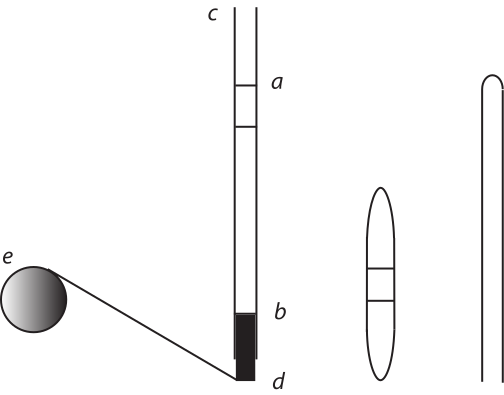
\includegraphics[width=0.5\textwidth]{images/37_3_95v1-v3}
%                        %\caption{Bildbeschreibung}
%                       % \end{wrapfigure}
%                        %\begin{wrapfigure}{l}{0.05\textwidth}                    
%             %   \includegraphics[width=0.05\textwidth]{images/37_3_95v3}
%                        %\caption{Bildbeschreibung}
%                        %\end{wrapfigure}
%                        %\begin{wrapfigure}{l}{0.05\textwidth}                    
%          %      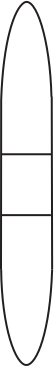
\includegraphics[width=0.05\textwidth]{images/37_3_95v4}
%          \\\rule[0cm]{2cm}{0cm}\textit{[Fig. 5] \rule[0cm]{1.3cm}{0cm}[Fig. 6]\rule[0cm]{0.2cm}{0cm} [Fig. 7]}
%                        %\caption{Bildbeschreibung}
%                        %\end{wrapfigure} 
%                        \end{center}
\pstart  Nota: Elateria\protect\index{Sachverzeichnis}{elaterium} eodem modo ponderant secundum  altitudinem ut \edtext{liquores. Mercurius}{\lemma{liquores.}\Afootnote{ \textit{ (1) }\ Si \textit{ (2) }\ Mercurius \textit{ L}}} in Tubo Torricelliano\protect\index{Sachverzeichnis}{Tubus!Torricellianus} delapsus aequiponderat pressioni aeris\protect\index{Sachverzeichnis}{pressio!aeris}, aer enim  ultra premi non patitur ab hac vi, addatur aliquid hanc vim,  ut si sit in Tubo receptaculum ex quo effundi possit Mercurius\protect\index{Sachverzeichnis}{mercurius} \edtext{additur ad compressionem.}{\lemma{Mercurius}\Afootnote{ \textit{ (1) }\ aut si per \textit{ (2) }\ additur ad compressionem. \textit{ L}}} \edtext{Et nihilominus,  puto, eadem Mercurii altitudo servabitur}{\lemma{compressionem.}\Afootnote{ \textit{ (1) }\ Ut si duplicetur Mercurius\protect\index{Sachverzeichnis}{mercurius|textit}, duplicabitur aeris compressio\protect\index{Sachverzeichnis}{compressio|textit}, semperque \textit{ (2) }\ Et [...] servabitur \textit{ L}}} \edtext{cujus rei}{\lemma{servabitur}\Afootnote{ \textit{ (1) }\ . Omne enim corpus  quod \textit{ (2) }\ cujus rei \textit{ L}}} in alio Elaterio\protect\index{Sachverzeichnis}{elaterium} quam aere experimentum  ita institui potest, sumatur Elaterium\protect\index{Sachverzeichnis}{elaterium}, hoc Mercurii\protect\index{Sachverzeichnis}{mercurius}  in Tubo aliquo (in summo \edtext{licet}{\lemma{}\Afootnote{licet \textit{ erg.} \textit{ L}}} aperti) delabentis pondereque\protect\index{Sachverzeichnis}{pondus} suo aliud corpus Elaterio\protect\index{Sachverzeichnis}{elaterium} tendendo applicatum deprimentis, pondere\protect\index{Sachverzeichnis}{pondus} tendatur. Esto Mercurius\protect\index{Sachverzeichnis}{mercurius} \textit{ab} in Tubo \textit{cd}  premens Embolum\protect\index{Sachverzeichnis}{embolus} exactum \textit{bd}  qui descendendo  rotam \textit{e} chorda \textit{ed} sibi connexam circumagit  et Elaterium\protect\index{Sachverzeichnis}{elaterium} tendit. Observetur altitudo ultra quam Mercurius\protect\index{Sachverzeichnis}{mercurius} descendere seu Elaterium\protect\index{Sachverzeichnis}{elaterium} tendere non potest. Infundatur plus Mercurii\protect\index{Sachverzeichnis}{mercurius} id quod plus est ultra tendet descendetque embolus\protect\index{Sachverzeichnis}{embolus} Mercuriusque\protect\index{Sachverzeichnis}{mercurius} magis, sed nihilominus summum Mercurii\protect\index{Sachverzeichnis}{mercurius}, quantumcunque tendatur Elaterium\protect\index{Sachverzeichnis}{elaterium}, nunquam  descendet infra \edtext{\textit{ab}. Hoc}{\lemma{\textit{ab}}\Afootnote{ \textit{ (1) }\ pondere\protect\index{Sachverzeichnis}{pondus|textit} simplici hoc non \textit{ (2) }\ . Hoc \textit{ L}}}  an verum sit experientia comprobandum est. Et rationis  videtur. Id enim quod additur solum agit, rem  suam, priore imbelli et contrapondio destructo. Agit  vero rem suam totam, quia tota %
%\begin{wrapfigure}{l}{0.4\textwidth}                    
 %               \includegraphics[width=0.4\textwidth]{images/37_3_95v1}\\\rule[0cm]{2.5cm}{0cm}\textit{[Fig. 7]}
                        %\caption{Bildbeschreibung}
  %                      \end{wrapfigure} 
                 vis Elaterii\protect\index{Sachverzeichnis}{elaterium} vicissim  a Mercurio\protect\index{Sachverzeichnis}{mercurius} destruitur seu contraponderatur.\pend
                 \pstart
                 Hinc  ita comprimit Elaterium\protect\index{Sachverzeichnis}{elaterium} ut infra \textit{ab} descendat, quasi  non affuisset, et proinde altitudo \textit{ab} remanet. Suppono  autem Elaterium\protect\index{Sachverzeichnis}{elaterium} esse ejus naturae ut continuo tendi possit  sine ruptura, elegans erit hoc experimentum et magnam  lucem dabit. Nam similiter si demas Mercurium\protect\index{Sachverzeichnis}{mercurius}, attolletur  sursum, sed nunquam ultra \textit{ab} ergo si pene totus  ademtus sit non attolletur tamen ultra \textit{ab} ac si totus adimatur, tum demum ipsum Elaterium\protect\index{Sachverzeichnis}{elaterium} plane liberatum  erit. Hinc sequitur altitudinem hanc determinari ab Elaterii\protect\index{Sachverzeichnis}{elaterium} statu naturali, seu embolum\protect\index{Sachverzeichnis}{embolus} \textit{db}  ad altitudinem \textit{a} assurrecturum esse si nihil  sit quod \textit{d} premat. Idem ergo si loco Mercurii\protect\index{Sachverzeichnis}{mercurius} vel aqua,  vel potius simplex pondus\protect\index{Sachverzeichnis}{pondus} adhibeatur, id enim nunquam  infra eam altitudinem descendet. Sed non erit idem  effectus si duplicetur Tubi latitudo, quia non ideo  angustiae oriuntur, ut in Hydrostaticis\protect\index{Sachverzeichnis}{hydrostatica} 
                   aequalitas inde altitudinum  ab angustiis illis oritur; nisi scilicet Elaterium\protect\index{Sachverzeichnis}{elaterium} istud  sit  liquidum, et Embolus\protect\index{Sachverzeichnis}{embolus} ipse fiat tanto latior, aut potius quia  liquidum nullus sit Embolus\protect\index{Sachverzeichnis}{embolus}. Ita Elaterium\protect\index{Sachverzeichnis}{elaterium} \edtext{quasi liquidum}{\lemma{}\Afootnote{quasi liquidum \textit{ erg.} \textit{ L}}} poterit esse lana. Mercurius\protect\index{Sachverzeichnis}{mercurius} enim latior, aut pondus\protect\index{Sachverzeichnis}{pondus} latius etiam latiorem lanae  partem comprimere conabitur ergo omnia eadem; et si non  latiorem, fortius tamen hinc contrapondium semper idem. Idem  experimentum fieri potest Aere compresso, cujus naturalis  amplitudo nobis cognita, semper enim descendet Mercurius\protect\index{Sachverzeichnis}{mercurius} aut aliud \edtext{pondus\protect\index{Sachverzeichnis}{pondus} praecise infra altitudinem  naturalem}{\lemma{pondus}\Afootnote{ \textit{ (1) }\ eousque de \textit{ (2) }\ praecise infra altitudinem  naturalem \textit{ L}}} quam aer posceret, sed in aere discrimen  quod turbatur aer extra tenditurque. Id ergo ut impediatur  fiat hoc machinamentum. Esto \edtext{Tubus}{\lemma{Esto}\Afootnote{ \textit{ (1) }\ pondus\protect\index{Sachverzeichnis}{pondus|textit} \textit{ (2) }\ Tubus \textit{ L}}} praelongus,  clausus utrinque pondere\protect\index{Sachverzeichnis}{pondus} prius immisso, sive id sit Mercurius\protect\index{Sachverzeichnis}{mercurius}, \edtext{aliusve liquor}{\lemma{}\Afootnote{aliusve liquor \textit{ erg.} \textit{ L}}} quod \edtext{optimum (quadrat enim lateribus  vitri) sive aliud corpus}{\lemma{optimum}\Afootnote{ \textit{ (1) }\ sive aliud exacte \textit{ (2) }\ (quadrat [...] corpus \textit{ L}}} vitri lateribus quadrans, hoc si  Tubo toti immittatur, primum \edtext{utrinque aperto}{\lemma{primum}\Afootnote{ \textit{ (1) }\   \textbar\ ab \textit{ erg.}\ \textbar\  altero latere \textit{ (2) }\ utrinque aperto \textit{ L}}}, inde  ubi Mercurius\protect\index{Sachverzeichnis}{mercurius} ad extremum pervenit utrinque clauso,
                   % \begin{wrapfigure}{l}{0.05\textwidth}                    
                %\includegraphics[width=0.05\textwidth]{images/37_3_95v2}
                        %\caption{Bildbeschreibung}
                       % \end{wrapfigure}
                        %\begin{wrapfigure}{l}{0.05\textwidth}                    
                %\includegraphics[width=0.05\textwidth]{images/37_3_95v3}
                        %\caption{Bildbeschreibung}
                        %\end{wrapfigure}
                        %\begin{wrapfigure}{l}{0.05\textwidth}                    
                %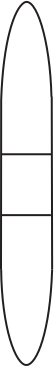
\includegraphics[width=0.05\textwidth]{images/37_3_95v4}
                        %\caption{Bildbeschreibung}
                        %\end{wrapfigure} 
                        et ita Mercurio\protect\index{Sachverzeichnis}{mercurius} descendendi libertas detur descendet per altitudinem  tantam quantam potest, fundum enim non pertinget et  ultra non descendet, nisi pondus\protect\index{Sachverzeichnis}{pondus} ejus augeatur, et quantum  augebitur \rule[-5mm]{0cm}{5mm}pondus\protect\index{Sachverzeichnis}{pondus} altius descendet, id est aerem magis reddet  difformem. Id est hinc \edtext{\edlabel{compi95v1}compressum}{\lemma{compressum}\xxref{compi95v1}{compi95v2}\Afootnote{ \textit{ (1) }\ hinc \textit{ (2) }\ illinc \textit{ L}}} illinc\edlabel{compi95v2}  dilatatum.  Augeatur ejus pondus\protect\index{Sachverzeichnis}{pondus} ut si in Tubo sint receptacula \edtext{ex quibus effunditur}{\lemma{}\Afootnote{ex quibus effunditur \textit{ erg.} \textit{ L}}} magis descendet,  et determinari calculo potest quantum descendere debeat  pro pondere\protect\index{Sachverzeichnis}{pondus} suo, semper autem ad eandem altitudinem  descendet idem pondus\protect\index{Sachverzeichnis}{pondus}, ubicunque in Tubo locetur, nisi locatum in summo  vi opus habeat ad aerem suum exprimendum si aere non sit  purgatum, at si aerem semel expresserit, descendet eodem  modo, antea suspensum. Descendet inquam sed simul suspensum  manebit, quod si diminuatur continue Mercurius\protect\index{Sachverzeichnis}{mercurius}, ut si magnete\protect\index{Sachverzeichnis}{magnes}  applicato intus cochleari\protect\index{Sachverzeichnis}{cochlea} exhauriatur, ne ponderet, pelletur  sursum, sed nunquam ultra altitudinem datam, quippe  naturalem, si augeatur pondus\protect\index{Sachverzeichnis}{pondus} nunquam infra altitudinem  datam descendet. Hinc colligi potest Mercurium\protect\index{Sachverzeichnis}{mercurius} totum  non descensurum, sed semper pendulum ex illa summitate  mansurum, in qua primo positus erat. Is enim est status aeris  inclusi naturalis seu uniformis. Impetu\protect\index{Sachverzeichnis}{impetus} lapsus nonnihil praevertet Mercurius\protect\index{Sachverzeichnis}{mercurius} sed  denuo repelletur. Et ut magis pateat veram causam horum effectuum  omnium esse difformitatis repugnantiam, non vero aeris Elaterium\protect\index{Sachverzeichnis}{elaterium}, et 
%                        \begin{wrapfigure}{l}{0.1\textwidth}                    
%        \protect\rule[0cm]{3mm}{0mm}        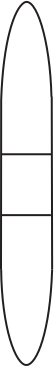
\includegraphics[width=0.033\textwidth]{images/37_3_95v4}\\\textit{[Fig. 8]}
%                        %\caption{Bildbeschreibung}
%                        \end{wrapfigure} 
                        aerem non minus repugnare dilatanti quam comprimenti  aperiatur sursum \edlabel{tubu95v1}Tubus. 
                        \edtext{Quid fiet?\edlabel{tubu95v2}}{\lemma{Tubus}\xxref{tubu95v1}{tubu95v2}\Afootnote{ \textit{ (1) }\ , Mercurius\protect\index{Sachverzeichnis}{mercurius|textit} violenter sursum feretur \textit{ (2) }\ .  Quid fiet? \textit{ L}}} Aer intrabit, et dilatatus in ordinarium statum abibit  \edtext{sed non enim  satis virium habet, compressus in fundo ad Mercurium elevandum}{\lemma{sed}\Afootnote{ \textit{ (1) }\ partim \textit{ (2) }\ abibit etiam \textit{ (3) }\ quaeritur an compresso fundi elevato  ita puto. Externus enim nullam vim passus non conabitur  ad restitutionem, et ita toti aeris   \textbar\ liberi \textit{ erg.}\ \textbar\  gravitati\protect\index{Sachverzeichnis}{gravitas|textit} praevalebit vis Elastica\protect\index{Sachverzeichnis}{vis!elastica|textit} inclusi, Mercuriusque\protect\index{Sachverzeichnis}{mercurius|textit} eousque elevabitur dum \textit{ (4) }\ non [...] elevandum \textit{ L}}};  ergo \edtext{an}{\lemma{an}\Afootnote{ \textit{ erg.} \textit{ L}}} tunc Mercurius\protect\index{Sachverzeichnis}{mercurius} magis etiam clauso denuo vitro comprimetur,  ita puto, perinde ac si totus aer utrinque esset aequaliter  compressus, Mercurius\protect\index{Sachverzeichnis}{mercurius} aequali facilitate in eo descenderet  quam in ordinario. Etsi enim alioquin aer compressus  jam difficillime comprimatur, id tamen totum fit a sola repugnantia difformitatis, quae hic minor, et ubi uterus compressus \edtext{nulla. Auferatur a Tubo Torricelliano}{\lemma{nulla.}\Afootnote{ \textit{ (1) }\ Hinc  \textit{(a)}\ cum \textit{(b)}\ in Tubo Torricelliano\protect\index{Sachverzeichnis}{Tubus!Torricellianus|textit} quia \textit{ (2) }\ Auferatur a Tubo Torricelliano \textit{ L}}} vas subjectum stagnans \edtext{postquam facta}{\lemma{stagnans}\Afootnote{ \textit{ (1) }\ eo momento, quo \textit{ (2) }\  postquam facta \textit{ L}}} descensio, Mercurius\protect\index{Sachverzeichnis}{mercurius} non effluet. \edtext{(Hoc videndum.)}{\lemma{}\Afootnote{(Hoc videndum.) \textit{ erg.} \textit{ L}}}  Agglutinetur eidem Tubo Torricelliano\protect\index{Sachverzeichnis}{Tubus!Torricellianus} a vase exemto  alius Tubus, Mercurius\protect\index{Sachverzeichnis}{mercurius} non ultra descendet, sed in Tubo  suspensus \edtext{manebit. Ut Mercurius in aqua  positus suspensus manet}{\lemma{manebit.}\Afootnote{ \textit{ (1) }\ Hinc sequitur ut Mercurius\protect\index{Sachverzeichnis}{mercurius|textit} in Tubo  maneat suspensus \textit{ (2) }\ Item attollatur \textit{ (3) }\ Ut [...] manet \textit{ L}}} cum aqua est quaterdecies altior. Hinc  sequitur ut Mercurius\protect\index{Sachverzeichnis}{mercurius} in Tubo suspensus maneat ad altitudinem  determinatam, opus esse ut totum Tubum impleverit et  ex summa ejus altitudine sit lapsus. Nam si totum Tubum  non impleverit etsi ex summa ejus altitudine sit lapsus Mercurius\protect\index{Sachverzeichnis}{mercurius}  suspensus in Tubo manebit quod est novum Baroscopii\protect\index{Sachverzeichnis}{baroscopium} \edtext{in aere penduli}{\lemma{}\Afootnote{in aere penduli \textit{ erg.} \textit{ L}}} experimentum. Hujus rei vera ratio est, quia repugnantia ad  descensum majorem est repugnantia aeris contra difformitatem  nam si magis descenderet, majus in Tubo spatium ab eodem aere  replendum, exteriorque magis comprimendus. At si cum Tubo augeatur  etiam Mercurius\protect\index{Sachverzeichnis}{mercurius} seu vis cum onere\protect\index{Sachverzeichnis}{onus} tunc necesse est eadem omnia evenire  quantacunque sit Tubi altitudo. At cur statur infra 27. pollices? Esto totus tubus\protect\index{Sachverzeichnis}{Tubus!Torricellianus} \edtext{Torricellianus}{\lemma{Torricellianus}\Afootnote{\textbar\ cum vase \textit{ gestr.}~\textbar\ in \textit{ L}}} in aere clauso, evacuetur arte pars Mercurii\protect\index{Sachverzeichnis}{mercurius} in aerem liberum, eo  ipso ascendet reliquus, sed nunquam ultra altitudinem datam. (Quemadmodum si novus  inseratur, nunquam infra altitudinem datam sit descensurus) ergo si plane totus Mercurius\protect\index{Sachverzeichnis}{mercurius} evacuetur, necesse est tunc eo momento aerem redire in statum naturalem. Ecce ergo determinationem 27. pollicum. Idem si loco evacuationis aut insertionis potius aer intus in receptaculis superfundatur aut auferatur. Sed cur hi  27. pollices sunt\edtext{}{\lemma{}\Afootnote{sunt  \textbar\ semper \textit{ gestr.}\ \textbar\ status \textit{ L}}} status aeris naturalis seu cur tunc compressus esse  desinit? Ecce aliud experimentum: aufer arte ex Mercurio\protect\index{Sachverzeichnis}{mercurius} delapso vel  in vase stagnante tantundem aut amplius Mercurii\protect\index{Sachverzeichnis}{mercurius} quantum est suspensum, delabitur Mercurius\protect\index{Sachverzeichnis}{mercurius}, insere aliquid amplius ultra 27. pollices  assurget quantum est spatium quod occupat novum insertum sine  ejus discrimine. Quod ergo ultra comprimi non potest vera  ratio est a vi Elaterii\protect\index{Sachverzeichnis}{vis!elaterii} aerei cum gravitate\protect\index{Sachverzeichnis}{gravitas} Mercurii\protect\index{Sachverzeichnis}{mercurius}  collata. \edtext{Est enim vis Elaterii  aerei}{\lemma{collata.}\Afootnote{ \textit{ (1) }\ Ut enim Mercurio\protect\index{Sachverzeichnis}{mercurius|textit} vel pondere \protect\index{Sachverzeichnis}{pondus|textit} ad Elaterium\protect\index{Sachverzeichnis}{elaterium|textit} commune alligato determinata quaedam vis est, ex qua pondus\protect\index{Sachverzeichnis}{pondus|textit} datum \textit{ (2) }\ Est enim vis Elaterii  aerei \textit{ L}}} tanta, ut a tota massa\protect\index{Sachverzeichnis}{massa} incumbente non ultra se comprimi  patiatur\edtext{.  Ergo}{\lemma{patiatur}\Afootnote{ \textit{ (1) }\ , seu potius ut in tota massa\protect\index{Sachverzeichnis}{massa|textit} \textit{ (2) }\ , ergo a \textit{ (3) }\ , in statum illum qui \textit{ (4) }\ .  Ergo \textit{ L}}} suspendet quantum massae\protect\index{Sachverzeichnis}{massa} illi aequiponderat. Nam reliquus Mercurius\protect\index{Sachverzeichnis}{mercurius}\footnote{\textit{\"{U}ber} Mercurius: NB}
                         qui Tubum impleverat ultra hos pollices, produxit pondere\protect\index{Sachverzeichnis}{pondus} suo omnem difformitatem, compressitque  extra Tubum, distendit in Tubo; at qui ipsi massae\protect\index{Sachverzeichnis}{massa}  incumbenti aequalis est, is nihil agit, ac proinde non delabitur,  nam si delaberetur, et ipse produceret difformitatem, quod non  potest, cum a toto Elaterio\protect\index{Sachverzeichnis}{elaterium} aeris in summa ei obsistatur. Sequitur: